\documentclass[a4paper, 10pt]{article}
\usepackage[utf8]{inputenc}
\usepackage{verbatim}
\usepackage{listings}
\usepackage{graphicx}
\usepackage{a4wide}
\usepackage{color}
\usepackage{amsmath}
\usepackage{amssymb}
\usepackage[dvips]{epsfig}
\usepackage[toc,page]{appendix}
\usepackage[T1]{fontenc}
\usepackage{cite} % [2,3,4] --> [2--4]
\usepackage{shadow}
\usepackage{hyperref}
\usepackage{titling}
\usepackage{marvosym }
\usepackage{subcaption}
\usepackage[noabbrev]{cleveref}
\usepackage{wasysym}


\renewcommand{\topfraction}{.85}
\renewcommand{\bottomfraction}{.7}
\renewcommand{\textfraction}{.15}
\renewcommand{\floatpagefraction}{.66}
\renewcommand{\dbltopfraction}{.66}
\renewcommand{\dblfloatpagefraction}{.66}
\setcounter{topnumber}{9}
\setcounter{bottomnumber}{9}
\setcounter{totalnumber}{20}
\setcounter{dbltopnumber}{9}


\setlength{\droptitle}{-10em}   % This is your set screw

\setcounter{tocdepth}{2}

\lstset{language=c++}
\lstset{alsolanguage=[90]Fortran}
\lstset{basicstyle=\small}
\lstset{backgroundcolor=\color{white}}
\lstset{frame=single}
\lstset{stringstyle=\ttfamily}
\lstset{keywordstyle=\color{red}\bfseries}
\lstset{commentstyle=\itshape\color{blue}}
\lstset{showspaces=false}
\lstset{showstringspaces=false}
\lstset{showtabs=false}
\lstset{breaklines}
\title{FYS2150 - Report 1\\
Time and Frequency}
\author{Gunnar Lange\\ Username:gunnalan}
\date{}
\begin{document}
\maketitle
\begin{abstract}
\begin{center}
We present three methods to measure the oscillatory period of a simple pendulum (by measuring its length, by measuring with a stopwatch and by measuring with a photodiode) and two methods to measure the time taken for an hourglass to  elapse (by a pendulum and by a stopwatch). We compare these methods, both on their accuracy and on their precision. We find that the photodiode gives the lowest uncertainty for measuring the period of a pendulum, whereas a stopwatch gives the lowest uncertainty for measuring an hourglass. We find good agreement between our results in general, but note that the amplitude of the pendulum must be kept within certain limits to be reliable, and that the hourglass appears to have a slight asymmetry between the two bulbs. All raw data from these experiments are available on our \href{https://github.com/gunnarlan/FYS2150-Data/tree/Report1-Time-and-frequency/Report1/Experiment/Experimental_Data}{GIT-page.}\footnote{\url{https://github.com/gunnarlan/FYS2150-Data/tree/Report1-Time-and-frequency/Report1/Experiment/Experimental_Data}}
\end{center}
\end{abstract}
\section{Introduction}
The measurement of time is amongst the most fundamental experiments in physics, as an enormous amount of measurements are based fundamentally on the ability to accurately measure time. We present an investigation into the measuring of time. We attempt to measure the time elapsed whilst an hourglass empties, using both a stopwatch and the periodic motion of a simple pendulum. We compare and contrast these methods, including a discussion of the limitations and uncertainties in both methods.\\
\linebreak
Subsequently, we investigate the period of the simple pendulum directly. We compute the period of the pendulum from a theoretical approximation, and compare this compute value to the value attained by a stopwatch and the value attained with a photodiode used to measure the oscillatory period.\\
\linebreak
We first introduce the theory necessary for these experiments. We continue with a brief discussion of the methods. Then, we present the results, and finish with a comparison of the attained values and a discussion of the uncertainties and errors in the experiment
\section{Theory}
\subsection{Theoretical period of a simple pendulum}
A simple pendulum consists of a heavy mass (the pendulum 'bob'), attached to a string. This string is then attached to a suspension point, from which the bob can swing freely. In the idealized case that the mass of the string is utterly negligible and a small initial angular displacement from the minimum position, it can be shown that (see \cite{pendulum}) the period of the pendulum only depends on the length from the suspension point to the center of mass of the bob, $L$ and the gravitational acceleration, $g$, according to the formula:s
\begin{equation}\label{eq:Period_of_pendulum}
T\approx2\pi \sqrt{\frac{L}{g}}
\end{equation}
The theoretical justification of this equation relies on the fact that $\sin \theta \approx \theta$ for small values of $\theta$, where$\theta$ is the angular displacement from the equilibrium position. Thus this equation is incorrect for large angles. In this idealized case, equation \ref{eq:Period_of_pendulum} can be used to determine the period of a pendulum based exclusively on $L$, and the location of the pendulum (which determines $g$). 
\section{Methods}
\subsection{List of equipment}
\begin{itemize}
\item Hourglass
\item Pendulum bob made from aluminimum, with support for string
\item String
\item Suspension point for pendulum
\item Folding ruler, produced by Hultafors
\item Strip of silver tape 
\item 100MT, Stopwatch produced by Clas Ohlson
\item Voltage source, providing 15 V
\item Photodiode of type IR-TXRX
\item NI-USB-6211 Data Acquisition unit
\item Computer with internal clock
\end{itemize}

\subsection{Experimental set-up of the pendulum}
The experimental set-up of the pendulum is shown in figure \ref{fig:Experiment_setup1}.
\begin{figure}[ht!]
\centering
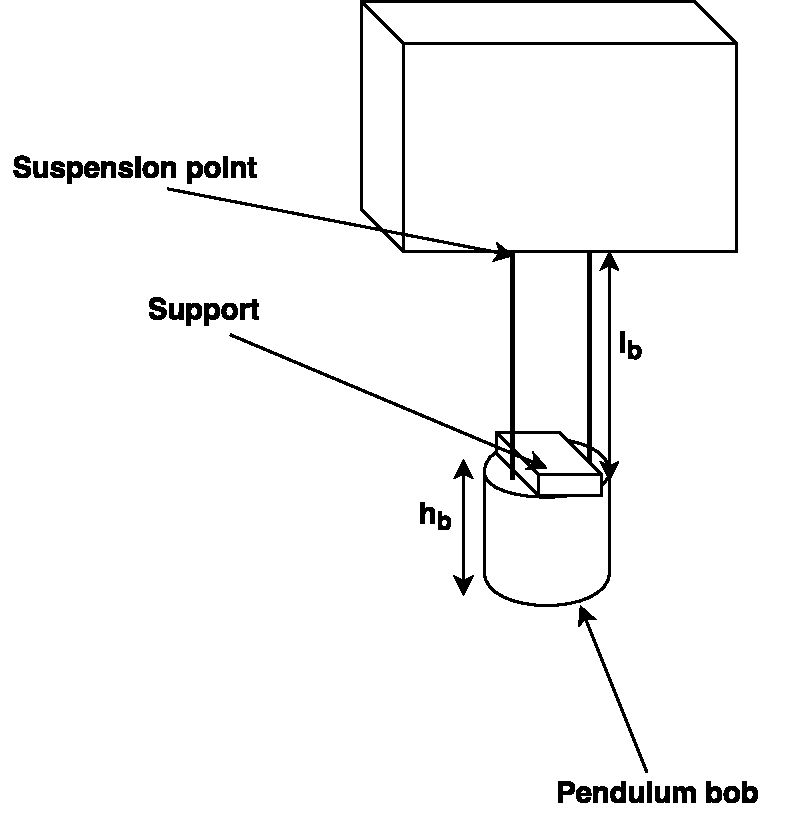
\includegraphics[scale=0.5]{FYS2150Lab1Diagram1.pdf}
\caption{Experimental set-up of the pendulum. For the values of the displayed parameters, see appendix \ref{ap:physical_parameters}.}\label{fig:Experiment_setup1}
\end{figure}
The string is fastened around the support of the pendulum bob, and attached at the suspension point. The pendulum is attached at two points, for increased stability. The oscillatory plane of the pendulum is normal to the figure.\\
\linebreak
We measured the length of the pendulum prior to any experiments, to determine the theoretical period from equation \ref{eq:Period_of_pendulum}. This is done by measuring the distance from the top of the cylindrical pendulum to the suspension point ($l_b$) with a folding ruler. We subsequently measure the height of the cylinder ($h_b$), and assume the cylinder to have homogeneous density, so that the center of mass is in the middle of the cylinder. Thus we calculate the effective length of the pendulum, $L$, by adding $l_b$ and $h_b/2$.\\
\linebreak
We begin by measuring the time elapsed by an hourglass, by counting the number of oscillations performed by the pendulum whilst the hourglass is running. We count once every time the pendulum passes the lowest point of its trajectory, and finally divide the count by two. We first set the pendulum in motion, and then start counting once the hourglass has been turned over and hits the table. We stop counting once the last grain of sand has disappeared from the top bulb of the hourglass.\\
\linebreak
We subsequently measure the period of the pendulum with a stopwatch. This is done by starting the pendulum from a small amplitude, and recording a lap on the stopwatch every time the pendulum bob passes the highest point of its trajectory. This enables us to take continuous measurements. We also measure the time elapsed by the hourglass with the stopwatch, starting the measurement when the hourglass hits the table and stopping the measurement when the last grain of sand vanishes from the top bulb.\\
\linebreak
Finally, we also measure the period of the pendulum with a photodiode.  This is done by connecting the photodiode to a 15 V voltage source, and connect it to the NI-USB-6211 data acquisition box, which measures  the time. The circuit diagram is shown in figure \ref{fig:Experiment_setup2} below:\\
\linebreak
\begin{figure}[ht!]
\centering
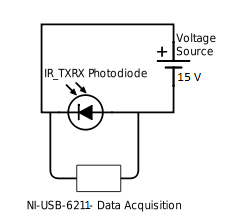
\includegraphics[scale=1]{schemeit-project.png}
\caption{Circuit diagram for photodiode measurements.}\label{fig:Experiment_setup2}
\end{figure}\\
The photodiode measures $5$ V constantly, except when there is something in front of it, where the voltage drops to $0$ V. We fasten a thin strip of silver tape to the bottom of the pendulum, and let the diode measure this strip. This improves the precision of the measurements, as the passing time of the pendulum is better defined.
We begin with a preliminary investigation into  the placement of the diode relative to the trajectory of the pendulum, for optimal data collection. Then we investigate the effect of changing the sampling frequency of the data acquisition tool and the amplitude of the pendulum, to see what effects this has on our measurements. 
\subsection{Uncertainties}
We approximated uncertainties based on what we observed in the experiments.\\
\linebreak
The Hulafors folding ruler had a stated uncertainty of $1$ mm per meter, and an additional $0.5$ m per joint used in measuring. This justifies the uncertainties stated in appendix \ref{ap:physical_parameters}.
\\
\linebreak
We observed that it was difficult to pin down the exact number of oscillations of the pendulum before the hourglass elapsed, and two counters disagreed slightly. It was also difficult to estimate anything below half a period. Therefore, the uncertainty in the number of periods taken before the hourglass elapsed was set to 1.\\
\linebreak
Wherever multiple measurements were performed, we set the uncertainty equal to the uncertainty of the mean (standard deviation of the measurements, divided by the square root of the number of measurements). These can then be compared.\\
\linebreak
Finally, in the case of equation \ref{eq:Period_of_pendulum}, we use standard error propagation. 
\section{Results}
\subsection{Results from the measurement of time by means of a pendulum}\label{results_pendulum_length}
The physical parameters of the pendulum, including their uncertainties, are presented in appendix \ref{ap:physical_parameters}. In table \ref{tab:time_measurement_pendulum} below, we present the number of times the bob passed it equilibrium point prior to the elapsing of the hourglass.\\
\linebreak
\begin{table}[ht!]
\centering
\caption{Measurements of the number of times the pendulum bob passes its equilibrium point before the hourglass elapses.}
\label{tab:time_measurement_pendulum}
\begin{tabular}{|l|l|}
\hline
\textbf{Measurement number}                              & \textbf{Number of equilibrium passes before hourglass elapses, $N$}             \\
\hline
1                                  & $229\pm 2$  \\
2		                            & $228 \pm 2$    \\
3									 & $232 \pm 2$   \\

\hline 
\end{tabular}
\end{table}\\
Giving:
$$\bar{N}=229\pm 1$$
Note, however, that this is the number of equilibrium passes, rather than the number of periods. Thus, the average number of periods, $\bar{P}$ before the hourglass runs out is:
$$\bar{P}=114.5 \pm 0.5$$
The effective length of the pendulum, $L$ is computed from table \ref{tab:physical_parameters_of_pendulum} in appendix \ref{ap:physical_parameters} to be:
$$L=58.5 \pm 0.4 \ \mathrm{cm}$$
Where a closer explanation of the uncertainty can be found in appendix \ref{ap:uncertainty_in_length}. The appropriate value for the gravitational constant $g$ can be found in \cite{gravity} to be:
$$g = 9.819\ \mathrm{m s^{-2}}$$
Where we assume that the uncertainty in this value is insignificant. 
The theoretical period, $T$ of the pendulum is then, using equation \ref{eq:Period_of_pendulum}:
$$T=1.534 \pm 0.005 \ \mathrm{s}$$
So that the average time taken by the hourglass, $\bar{t}_1$ is, with this method, given by:
$$\bar{t}_1=176 \pm 1\ \mathrm{s}$$
\subsubsection{Qualitative observations}
We note that,as shown in figure \ref{fig:Experiment_setup1}, the pendulum is suspended at the points. This made the estimation of the suspension point somewhat tricky, as it was not entirely certain that the pendulum was even level. It was also difficult to precisely estimate where in its trajectory the pendulum started as we turned the hourglass. Therefore, we decided to count equilibrium passes, rather than maxima, to count twice per oscillation. 
\subsection{Results from the measurement of time by means of a stopwatch}
\subsubsection{Results from measuring the period of a pendulum using a stopwatch}
The results from our measurements of the period of our pendulum, using a stopwatch, are shown in figure \ref{fig:Experiment_2} below. The raw data can be found on our \href{https://github.com/gunnarlan/FYS2150-Data/tree/Report1-Time-and-frequency/Report1/Experiment/Experimental_Data}{GIT-page.}\footnote{\url{https://github.com/gunnarlan/FYS2150-Data/tree/Report1-Time-and-frequency/Report1/Experiment/Experimental_Data}}.
\begin{figure}[ht!]
\centering
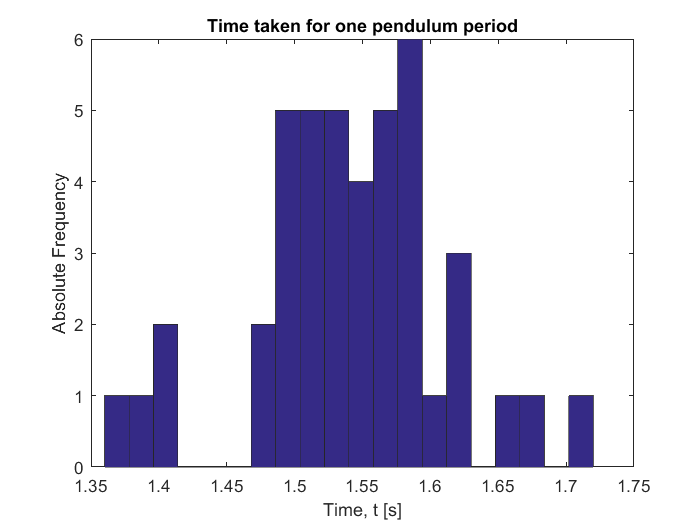
\includegraphics[scale=0.7]{Experiment2.png}
\caption{Histogram of the different times for the pendulum, measured using a handheld 100MT stopwatch produced by Clas Ohlson}\label{fig:Experiment_2}
\end{figure}\\
This gives the average period of the pendulum,$\bar{T}_2$ as:
$$\bar{T}_2=1.54  \pm 0.07 \ \mathrm{s}$$
\newpage
\subsubsection{Results from the measurement of the time taken for an hourglass to elapse using a stopwatch}
The raw data for the measurements of the hourglass using the stopwatch are also found on our \href{https://github.com/gunnarlan/FYS2150-Data/tree/Report1-Time-and-frequency/Report1/Experiment/Experimental_Data}{GIT-page.}\footnote{\url{https://github.com/gunnarlan/FYS2150-Data/tree/Report1-Time-and-frequency/Report1/Experiment/Experimental_Data}}. The histogram of this is shown below:
\begin{figure}[ht!]
\centering
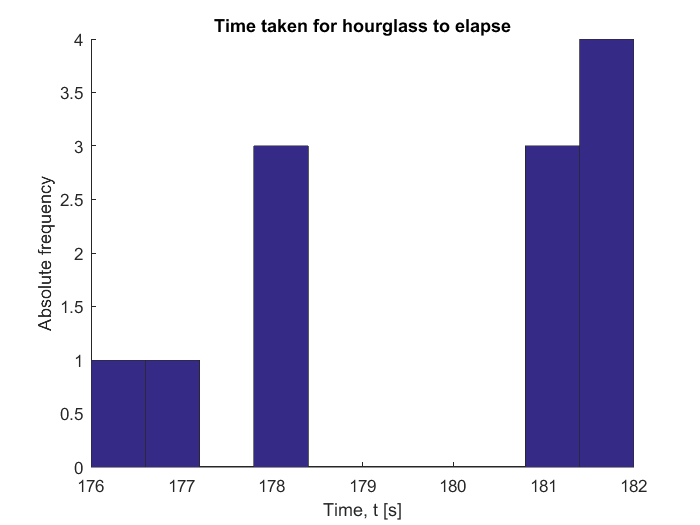
\includegraphics[scale=0.7]{Experiment2_2.png}
\caption{Histogram of the different times for the hourglass, measured using a handheld 100MT stopwatch produced by Clas Ohlso}\label{fig:Experiment_2_2}
\end{figure}\\
The average time for the hourglass to elapse, $\bar{t}_2$ is given by:
$$\bar{t}_2 = 179.8 \pm 0.6 \ \mathrm{s}$$
\subsubsection{Qualitative observations}\label{Discarding_stopwatch}
One important thing to note for figure \ref{fig:Experiment_2_2} is that, due to humman failure, some runs had to be discarded. This was because the hourglass ran out without the experimenter noticing, resulting in times that were far too long and were therefore discarded.
\subsection{Results from the measurement of the pendulum period by means of a photodiode}
The results from the photodiode experiment, using small initial amplitudes and a sampling frequency of $25\ \mathrm{kHz}$ is shown in the figure below:\newpage
\begin{figure}[ht!]
\centering
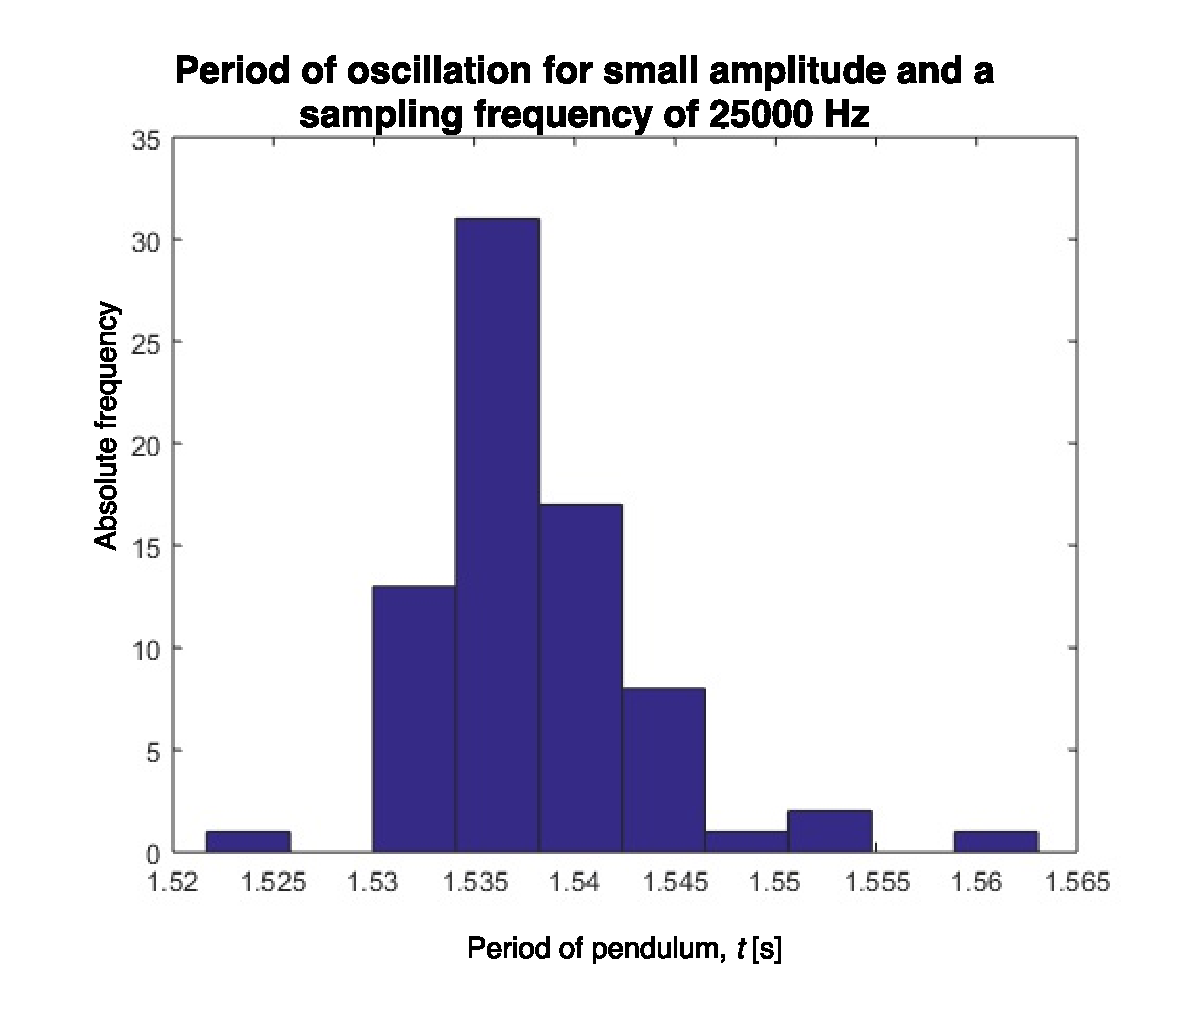
\includegraphics[scale=0.7]{Experiment2_3_small_high.pdf}
\caption{Histogram of the different times for the period of the pendulum, measured using a photodiode with large ($25$ kHz) sampling frequency and small initial amplitude of the pendulum.}\label{fig:Experiment_2_3_small_high}
\end{figure}Keeping a small amplitude but decreasing the sampling frequency to $2500 \ \mathrm{Hz}$ gave the following data:\newpage
\begin{figure}[ht!]
\centering
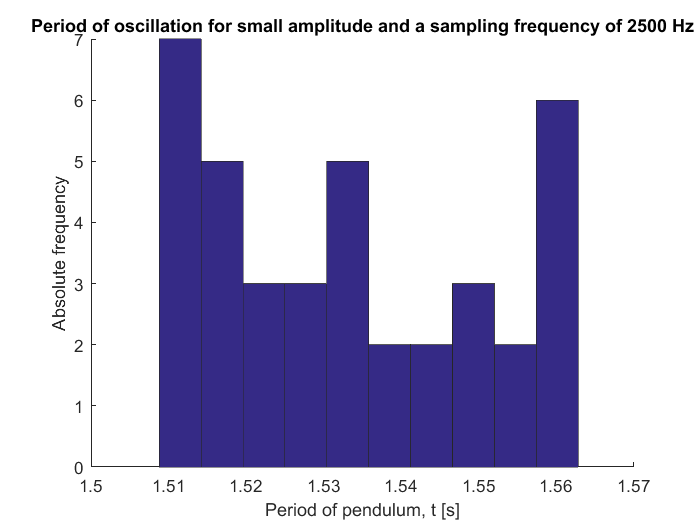
\includegraphics[scale=0.6]{Experiment2_3_small_low.png}
\caption{Histogram of the different times for the period of the pendulum, measured using a photodiode with a lower ($2.5$ kHz) sampling frequency and small initial amplitude of the pendulum.}\label{fig:Experiment_2_3_small_low}
\end{figure}
Finally, keeping the large sampling frequency, but increasing the amplitude gave the following histogram:\\
\begin{figure}[ht!]
\centering
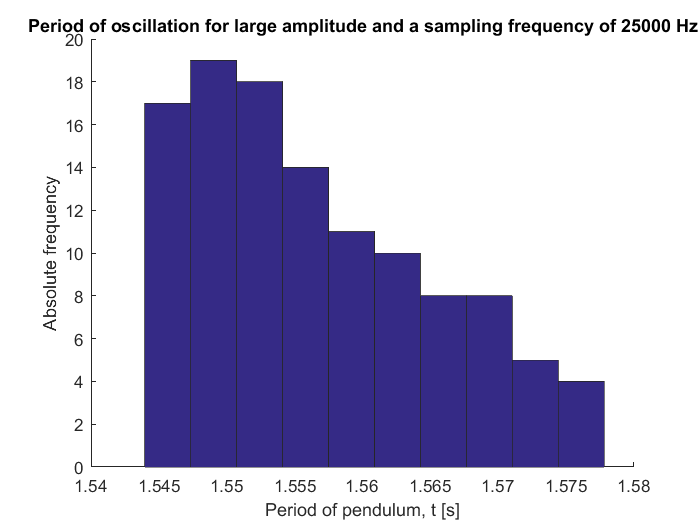
\includegraphics[scale=0.6]{Experiment2_3_large_high.png}
\caption{Histogram of the different times for the period of the pendulum, measured using a photodiode with a high ($25$ kHz) sampling frequency and a large initial amplitude of the pendulum.}\label{fig:Experiment_2_3_large_high}
\end{figure}
\newpage
For later discussion, we also include a time plot of figure \ref{fig:Experiment_2_3_large_high}. As all measurements were taken continuously (during the same pendulum swing), this gives an equivalent representation of the data.\\
\begin{figure}[ht!]
\centering
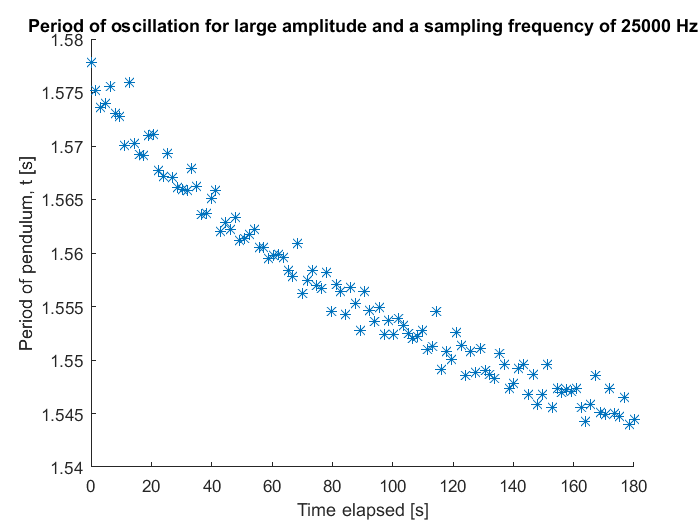
\includegraphics[scale=0.7]{Experiment2_3_large_high_time.png}
\caption{Histogram of the different times for the period of the pendulum, measured using a photodiode with a high ($25$ kHz) sampling frequency and a large initial amplitude of the pendulum, for a total of three minutes.}\label{fig:Experiment_2_3_large_high_time}
\end{figure}
\linebreak
A summary of the mean quantities from these experiments, combined with their uncertainties, is shown in table \ref{tab:mean_times_photodiode} below.
\begin{table}[hb!]
\centering
\caption{Mean times from the photodiode}
\label{tab:mean_times_photodiode}
\begin{tabular}{|l|l|}
\hline
\textbf{Experiment}                              & \textbf{Mean time}                 \\
\hline
Small amplitude, high sampling frequency, $T_{sh}$     & $1.534 \pm 0.002 \ \mathrm{s}$ \\
Small amplitude, low sampling frequency, $T_{sl}$ & $1.533 \pm 0.003\ \mathrm{s}$   \\
Large amplitude, high sampling frequency, $T_{lh}$ & $1.5566 \pm 0.0008\ \mathrm{s}$   \\
\hline 
\end{tabular}
\end{table}
The raw data for these experiments is available from our \href{https://github.com/gunnarlan/FYS2150-Data/tree/Report1-Time-and-frequency/Report1/Experiment/Experimental_Data}{GIT-page.}\footnote{\url{https://github.com/gunnarlan/FYS2150-Data/tree/Report1-Time-and-frequency/Report1/Experiment/Experimental_Data}}
\subsubsection{Qualitative observations} \label{photodiode_qualitat}
We tested a multitude of positions for the diode, relative to the trajectory of the pendulum. At the top of the trajectory, the photodiode sometimes failed to register an oscillation, as the amplitude decreased slightly with time. Further down, the photodiode would sometimes register an oscillation twice(once on the way up and once on the way down). It was therefore decided to place the sensor near the bottom point of the pendulum. This was no problem, as long as the sampling frequency was large enough.
\section{Discussion}
\subsection{Comparing the results}
Comparison of the theoretical period of the pendulum, $T$, and the period measured by the stopwatch, $\bar{T}_2$ shows good agreement. $T$ is contained inside the uncertainty interval of $\bar{T}_2$. Thus the values are in agreement. This period may also be compared with the measurements made by the photodiode, shown in table \ref{tab:mean_times_photodiode}. Note that the theoretical value, $T$, is within the uncertainty interval of $T_{sh}$ and $T_{sl}$ (small amplitude and both high and low sampling frequency). However, the period is not within the uncertainty of $T_{lh}$ (large amplitude, high sampling frequency). This suggests that there may be a systematic error in the large amplitude. Figure \ref{fig:Experiment_2_3_large_high_time} also suggest this, as the period varies systematically with time. This is explored further in section \ref{Uncertainty_in_pendulum_period}.\\
\linebreak
Comparison of the time taken for the hourglass to elapse, $\bar{t}_1$ and $\bar{t}_2$, shows a lack of agreement. Whilst the numbers are similar, they are not within the uncertainty of each other. This suggests that there may be additional sources of error, that have not yet been accounted for. This is discussed further in section \ref{Uncertainty_in_pendulum}.
\subsection{Uncertainties and discussion of errors}
A significant number of sources contribute to the uncertainty in this experiment, and have to be addressed.\\
\subsubsection{Calculating the period of the pendulum from its length}\label{pendulum_support}
The main source of error when estimating the period of the pendulum, $T$ from its length, $L$ was presumably in determining the exact position of the center of mass of the bob. The bob had an additional support for the string at the top, which was made out of the same material as the bob. This presumably shifted the position of the center of mass away from the center of the cylinder, further upwards. However, in lack of a more precise way to measure the center of mass, this systematic error was simply added to the uncertainty, in a way described in appendix \ref{ap:uncertainty_in_length}.\\
\linebreak
Another problem was the measuring stick itself. The uncertainty as found in the reference notes was approximately $1$ mm. The fact that the exact location of the suspension point of the pendulum was somewhat difficult to estimate, due to its double suspension, presumably incurred another contribution to the random error of this measurement. However, both of these sources of error appear to be much smaller than the error due to the incorrect estimation of the center of mass, and were therefore not investigated further.\\
\linebreak
One final problem with estimating the period may have been the value of $g$, whose precision is not known. However, as this is a reference value, and the experiments were performed in the city stated in the reference, this error was assumed negligible.
\subsubsection{Estimating the time elapsed on an hourglass}\label{Uncertainty_in_pendulum}
In estimating the time elapsed by an hourglass by means of a pendulum, the main uncertainty originates from determining the number of oscillations of the pendulum. We counted one passes every time the pendulum passed its lowest point, and then divided this count by two. The small-angle approximation meant that we required small amplitudes, which made determining the exact position of the pendulum, both at the beginning and at the end of the measurement, difficult. We therefore initially added one period uncertainty to each individual measurement, and the uncertainty of the mean showed that this was indeed required.\\
\linebreak
Further sources of error were the approximations made by our formula. Equation \ref{eq:Period_of_pendulum} only holds for small angles, and assumes no dissipative forces. These assumptions were clearly not entirely correct. We attempted to account for this by choosing small amplitudes, to justify the small-angle approximation. This also implies a lower average velocity, and as most dissipative forces scale with the velocity, this should also minimize the effect of dissipative forces. As such, we assumed these factors to be negligible.\\
\linebreak
The main contribution to the uncertainty when estimating the time elapsed on the hourglass by means of a stopwatch was the start-and stopping time. This was not always easy to determine precisely, and incurred the loss of some measurements, as stated in section \ref{Discarding_stopwatch}. Additional issues may have been the slamming of the hourglass on the table when turning it, which may have slightly accelerated the time.\\\linebreak
An interesting feature of figure \ref{fig:Experiment_2_2} is that the times are clearly not normally distributed. Instead, there appears to be a clear grouping into high times (181 seconds, 182 seconds) and lo times (176, 177 and 178 seconds). This may be indicative of a systematic error. The most likely explanation of this phenomenon may be that the hourglass was slightly asymmetric, so that the time for the sand to run out varied between the two bulbs of the hourglass. As some measurements were lost, due to forgetfulness (see section \ref{Discarding_stopwatch}), these do not have to be equally distributed. This may also explain the apparent disparity between the measurements made by the pendulum ($\bar{t}_1$) and the measurements made by the stopwatch ($\bar{t}_2$). It may be that $\bar{t}_1$ got two low times one high time, meaning that the average was low, whereas $\bar{t}_2$ clearly got more high times, implying that the average is higher. This corresponds well with the observed data, and may therefore be an explanation of the difference between $\bar{t}_1$ and $\bar{t}_2$.
\subsubsection{Estimating the period of the pendulum}\label{Uncertainty_in_pendulum_period}
When measuring the pendulum with a stopwatch, the most obvious source of error was the human reaction time. We measured at the extreme of the pendulum's trajectory, where its velocity was smallest, to get the most exact measurements possible. However, as explained in section \ref{Uncertainty_in_pendulum}, we required small angles, and therefore small amplitudes. This meant that it was difficult to estimate the period precisely, contributing to the random error. This is reflected by the fact that the uncertainty in $\bar{T}_2$ is much larger than the uncertainty in $T$ or in and of the periods from table \ref{tab:mean_times_photodiode}.\\
\linebreak
The earlier comments from section \ref{Uncertainty_in_pendulum} about the uncertainties inherit in the experiment of the pendulum, concerning small-angle approximations and dissipative forces, also apply to this part of the experiment.\\
\linebreak
The photodiode did not suffer from these human errors, as reflected by the much lower uncertainty. Instead, the main problem was ensuring that the diode registered every pass. As discussed in section \ref{photodiode_qualitat}, this was achieved by moving the sensor close to the bottom of the pendulum's trajectory. The sampling frequency had little impact on the precision of the measurement, as can be seen in table \ref{tab:mean_times_photodiode}, as long as the sampling frequency was sufficiently large to ensure that every pass of the pendulum was precisely recorded.\\
\linebreak
It is interesting to compare figure \ref{fig:Experiment_2_3_small_high}, \ref{fig:Experiment_2_3_small_low} and \ref{fig:Experiment_2_3_large_high}. Figure \ref{fig:Experiment_2_3_small_low} has a distribution that spikes at the corners. This may just be due to few data points. Alternatively, it could indicate that the sampling frequency was just slightly too low, so that the diode tended to slightly over- or underestimate the period. Figure \ref{fig:Experiment_2_3_small_high} shows a much more even distribution, which looks approximately Gaussian. This may just be due to the fact that  this figure has more data points. This could alternatively indicate that the larger sampling frequency did give a better representation of the data. Either way, as can be seen in table \ref{tab:mean_times_photodiode}, both measurements gave similar data. Finally, compare these to figure \ref{fig:Experiment_2_3_large_high}. This figure differs markedly, as there is a clear trend in the data - the distribution is much more skewed. To investigate this more carefully, we plot the measurements as a function of time in figure \ref{fig:Experiment_2_3_large_high_time}. This figure shows the problem quite clearly. The pendulum starts out with a large period, which quickly decreases. This seems to be an example of the small-angle approximation breaking down. Starting with a large amplitude, as was done here, implies that the small-angle approximation, giving equation \ref{eq:Period_of_pendulum}, is no longer valid. The period is no longer just a function of the length, but also of the amplitude. As can be seen in figure \ref{fig:Experiment_2_3_large_high_time}, the  period starts out as being quite large, but quickly decreases, asymptotically approaching the period estimated from equation \ref{eq:Period_of_pendulum}, $T$. Large amplitudes imply large velocity, and as such, the effect shown in figure \ref{fig:Experiment_2_3_large_high_time} shows dissipative forces decreasing the amplitude of the oscillations, so that the small-angle approximation becomes more valid with time. This also explains the disparity between $T$ and $T_{lh}$. Note that the low uncertainty of $T_{lh}$ is due to the large number of data points, not the constancy of the measurements, and therefore cannot be used to directly compare $T_{lh}$ to the other measurements. 
\section{Conclusion}
\subsection{Summary}
Most of our results are consistent with each other. It seems safe to say, at the very least, that the period of pendulum is close to 1.54 seconds, at least for small angles. We have observed that the small angle approximation is vital for these results, and that the approximation affects the results to an appreciable degree. The other effects, such as dissipative forces, seems negligible in comparison - at least if the pendulum is heavy enough. This is important to keep in mind if one were to use the pendulum as an accurate time keeping device.\\
\linebreak
The results from the investigation into the elapsing time of the hourglass seem less conclusive. It seems safe so assert that the time, $t$ is close to $180$ seconds, but the uncertainty on both sides would have to be several seconds, and it seems that it is important to keep track of which of the bulbs is at the top.
\subsection{Outlook}
There is quite some room for future investigation in this experiment. In particular, it may be of interest to investigate quantitatively the effect seen in figure \ref{fig:Experiment_2_3_large_high_time}, showing a decrease of the period with time, to see to what extent the small angle approximation influenced the obtained results.\\
\linebreak
It may also be of further interest to investigate the asymmetry of the hourglass, if this is indeed the explanation of the data. If so, then it may be necessary to mark the hourglass, to distinguish the two sides, before it can be used as an accurate time-taking device.
\bibliography{Report1}{}
\bibliographystyle{plain}
\pagebreak
\begin{appendices}
\section{Physical parameters of the pedulum}\label{ap:physical_parameters}
\begin{table}[ht!]
\centering
\caption{Physical parameters of the pendulum}
\label{tab:physical_parameters_of_pendulum}
\begin{tabular}{|l|l|}
\hline
\textbf{Quantity}                              & \textbf{Value}                 \\
\hline
Height of bob, $h_b$                                  & $10.20\pm 0.05  \mathrm{cm}$  \\
Length from top of the bob to suspension point $l_b$ & $53.4 \pm 0.1 \mathrm{cm}$   \\
\hline 
\end{tabular}
\end{table}
\section{Deriving the uncertainty in the length measurements}\label{ap:uncertainty_in_length}
As stated in \ref{pendulum_support}, we noted that the bob was supported by a rather heavy support in which to tread the wire suspending the pendulum, as shown schematically in figure \ref{fig:Experiment_setup1}. Measurements of the volume of this support gave (assuming it to have a similar density as the bob) that the support made up about $7\%$ of the mass of the pendulum. As this mass was on top, our estimate of the center of mass of the pendulum may have been off by as much as $7\%$. The length of the pendulum, $L$ was estimated as (for an explanation of the symbols, refer to table \ref{tab:physical_parameters_of_pendulum}): 
$$L=\frac{h_b}{2}+l_b$$
Adding a $7\%$ uncertainty to $h_b/2$, and assuming these uncertainties to be additive, gives the total uncertainty as:
$$\Delta L = \sqrt{\left(\frac{h_b}{2}\cdot 0.07\right)^2+ \left(\Delta\frac{h_b}{2}\right)^2+(\Delta l_b)^2} \approx 0.4 \ \mathrm{cm} $$
Which explains the uncertainty stated in \ref{results_pendulum_length}.
\end{appendices}
\end{document}